\chapter{Parallel Merging Algorithm Implementation on GPU}\label{chap:implementation}
Compared to CMPs, GPUs have more threads and larger memory bandwidth 
for the purpose of massive parallelism. 
However, a direct translation of a parallel algorithm suits CMPs
may not run efficiently on GPUs. 
To explore massive parallelism on GPUs, we need to coordinate 
the memory access pattern, make full use of the shared memory, reduce the thread 
divergence, improve the load balance for different processing units, and create enough 
parallelism.

As the first step, we implement this parallel merge algorithm on GPU without any 
GPU-specific optimization. We 
name it \textbf{naive parallel merge}. More details about naive parallel merge 
are described in section \ref{sect:naive}. 

However, the naive parallel merge did not incorporate any GPU-specific optimizations, 
which is critical to improve the application performance that runs on GPU.  
We implement an optimized GPU version that utilizes shared memory as a scratch pad to make the 
accesses to global memory coalesced. We name it \textbf{single buffer 
parallel merge}. More details about single buffer parallel merge are described in section 
\ref{sect:single}. 

In single buffer parallel merge, we only consume half of the 
data we load into the shared memory. The other half is wasted. 
To better utilize the data we load into shared memory, we implement a third version. And we 
name it \textbf{double buffer parallel merge}. We describe more details about double buffer 
parallel merge in section \ref{sect:double}.

%%%%%%%%%%%%%%%%%%%%%%%%%%%%%%%%%%%%%%%%%%%%%%%%%%%%%%%%%%%%%%%%
%   
%   Naive Parallel Merge
%
    \section{Naive Parallel Merge}\label{sect:naive}
    In naive parallel merge, we copy the input arrays $A[\,]$ and $B[\,]$ from host to device global 
    memory first.
    Then each thread calculates the thread index ($r$) and total number of threads ($p$) 
    using $t\_id = blockIdx.x * blockDim.x + threadIdx.x$ and $t\_num = gridDim.x * blockDim.x$ 
    respectively. Based on $t\_id$ and $t\_num$, each thread calculates the output range it is 
    going to produce, and uses the output range as the input to the co-rank function to identify the 
    corresponding input ranges. After getting the input ranges, all threads can start to merge 
    independently by calling the sequential merge function in parallel and writing the result
    to $C[\,]$ in device global memory. Finally, we copy $C[\,]$ from device global memory back to the host.

    Figure \ref{fig:naive} shows an example of naive parallel merge. $A[\,]$, $B[\,]$ and $C[\,]$ 
    are in device global memory. This example shows the work of one thread. After identifying
    its output range($C[\,]$) and input ranges($A[\,]$, $B[\,]$), it uses sequential merge to write the
    result to $C[\,]$. All the threads will run in parallel and produce the result for the entire 
    output array $C[\,]$.   

    \begin{figure}[!h]
    \begin{center}
    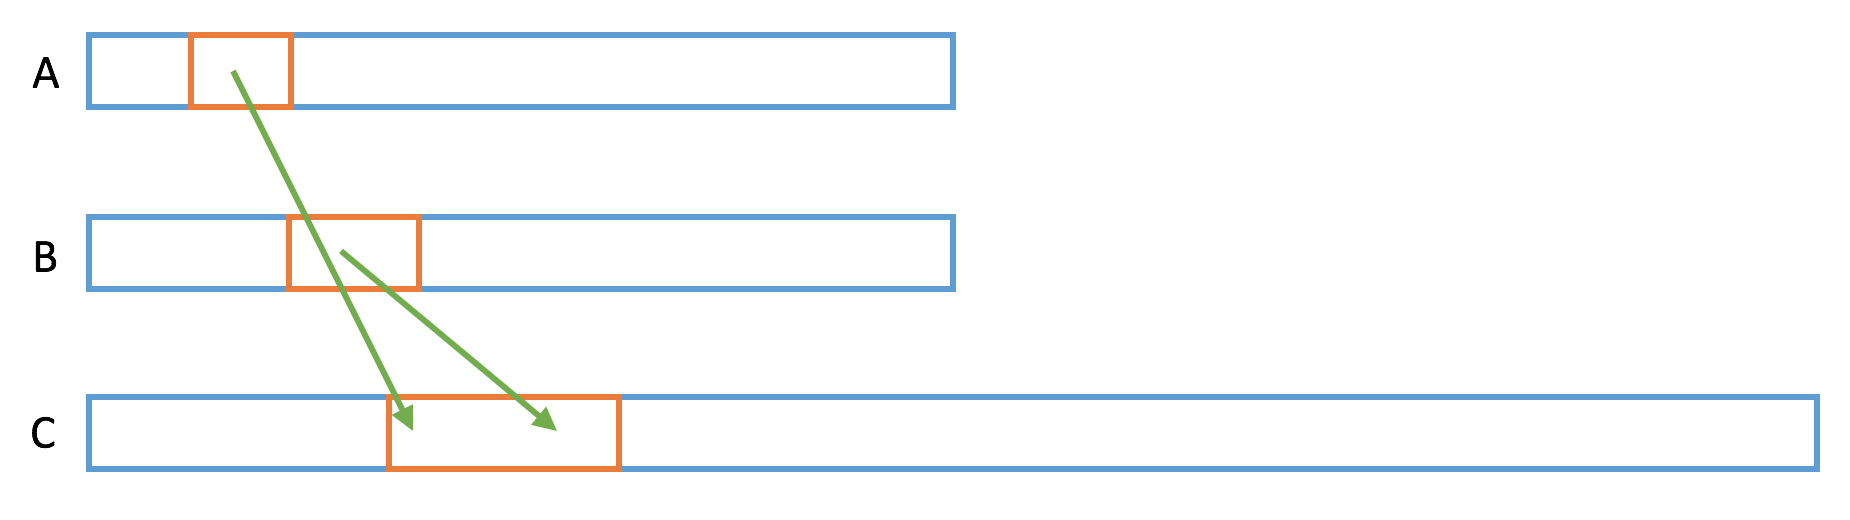
\includegraphics[width=\textwidth]{naive.png}
    \end{center}
    \caption{{\label{fig:naive}} Naive Parallel Merge}
    \end{figure}

    The performance of naive parallel merge on titan-z is shown in Figure \ref{fig:naive_evaluation}.
      
    \begin{figure}[!h]
    \begin{center}
    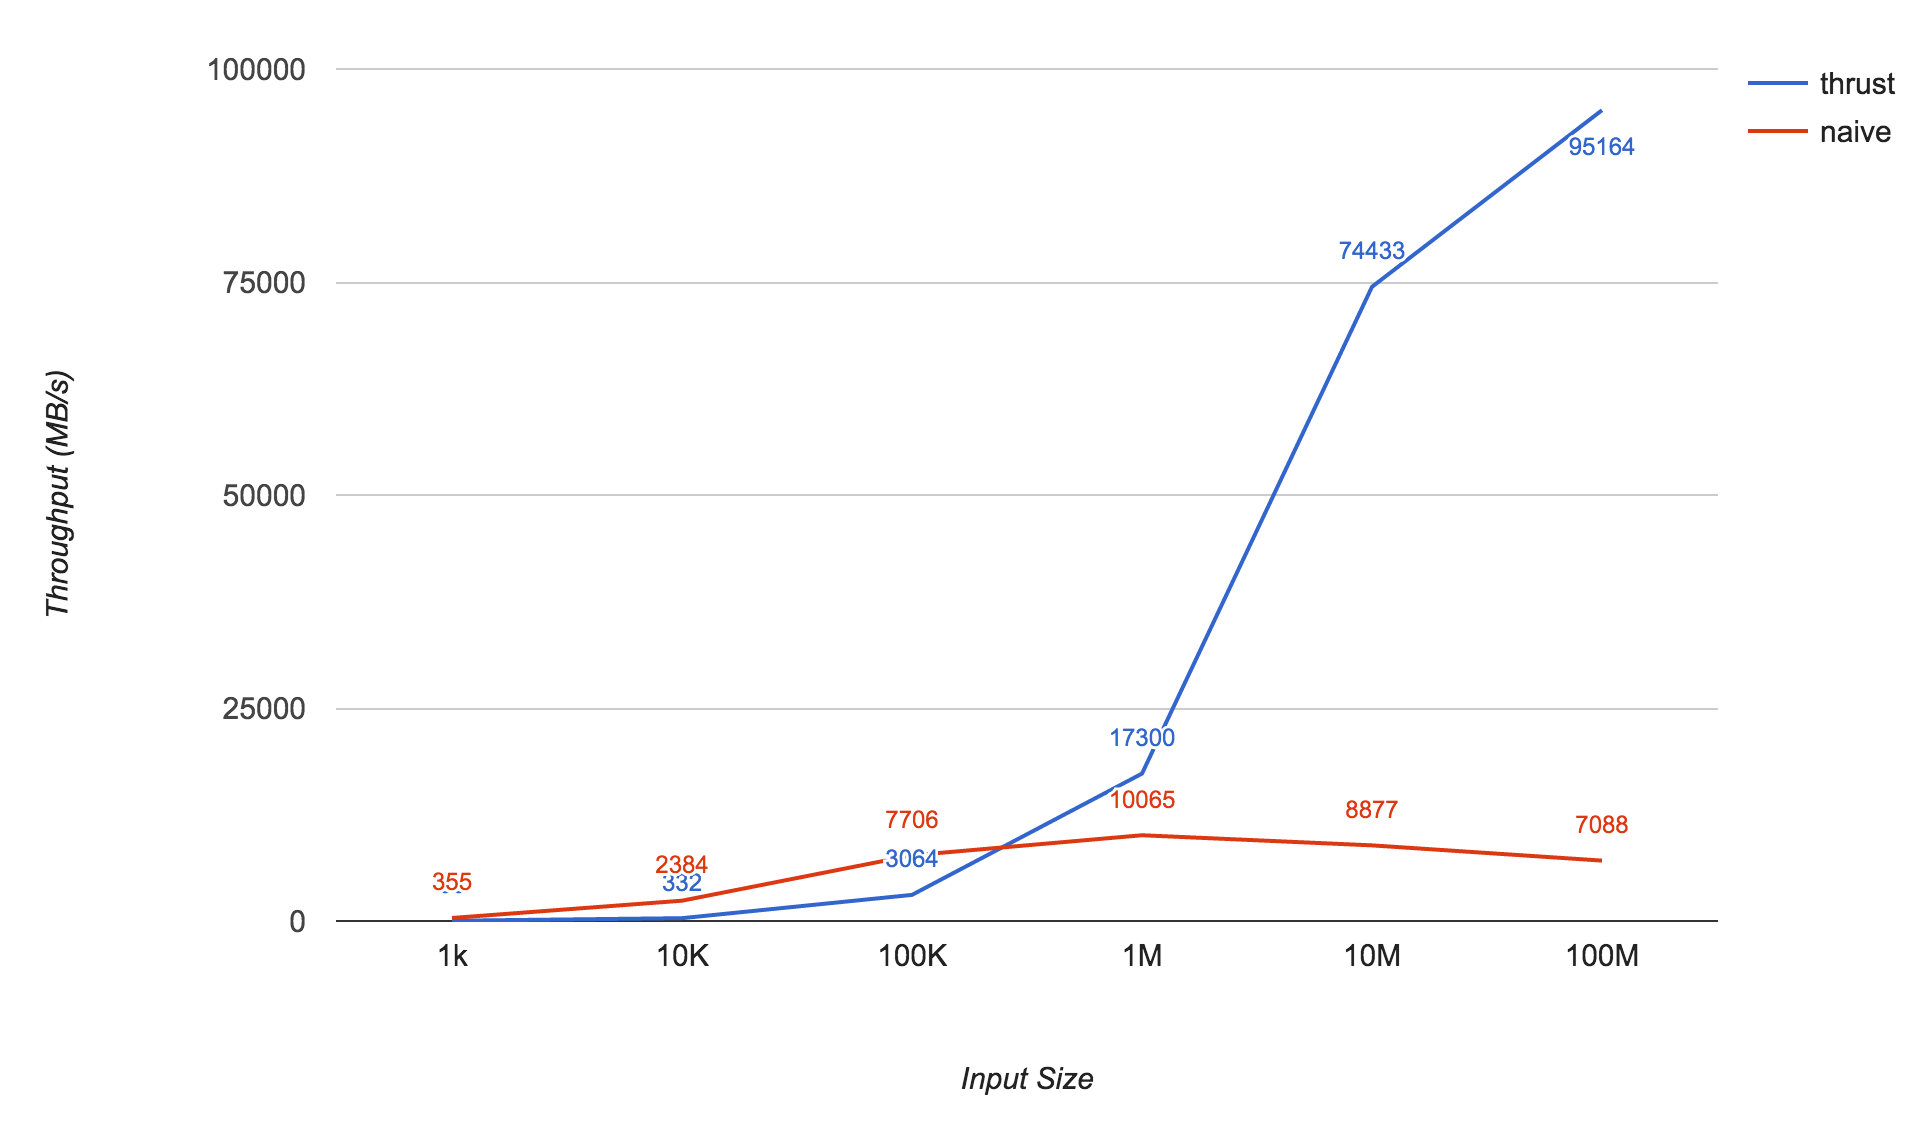
\includegraphics[width=\textwidth]{naive_evaluation.png}
    \end{center}
    \caption{{\label{fig:naive_evaluation}} Performance of Naive Parallel Merge on Titan-Z}
    \end{figure}

    In naive parallel merge, both the co-rank function and merge function run on the global memory. Due to 
    the nature of the co-rank function, in which each thread is doing a binary search for its own input 
    index, the memory access pattern is not coalesced. The memory access pattern for merger function
    is not coalesced either. For these reasons, although naive parallel merge is faster than thrust merge 
    for certain input size, it still underutilizes the memory 
    bandwidth offered by GPU and therefore did not achieve the optimal overall performance.


%%%%%%%%%%%%%%%%%%%%%%%%%%%%%%%%%%%%%%%%%%%%%%%%%%%%%%%%%%%%%%%%
%   
%   Single Buffer Parallel Merge
%
    \section{Single Buffer Parallel Merge}\label{sect:single}
    The memory access pattern in naive parallel merge is not coalesced. To improve the memory 
    throughput on GPU, coalesced global memory accesses pattern are critical. For this reason, 
    we use shared memory on GPU to make the access pattern to global memory coalesced in single
    buffer parallel merge. Single buffer parallel merge works as follows: Co-rank function is
    run in two levels, block level and thread level. In the block level, all the threads in 
    the same block do the same searching. Each thread calculates the block index and total 
    number of blocks using $b\_id = blockIdx.x$ and $b\_num = gridDim.x$ respectively. 
    Based on $b\_id$ and $b\_num$, all threads within the same block calculate the output range 
    that block is going to produce, and use the output range as the input to the co-rank function 
    to identify the corresponding input ranges for that block. The co-rank function is run on 
    global memory in the block level.  
    After knowing the input ranges for the block, all threads in the block cooperatively load the 
    input to the shared memory. In this way, we can guarantee that the global memory access 
    pattern is coalesced. 

    However, the shared memory may not be large enough to hold all the input data. 
    So we create a loop. In each iteration, we load $x$ elements from input array A and 
    $x$ elements from input array B into the shared memory. This will produce $x$ (not $2x$) 
    elements to the output array C. Because in extreme cases, all the output may come from 
    one of the input array, we waste half of the data loaded into the shared memory.
 
    Then we run the co-rank function in thread level. Threads in a block will merge $x$ 
    elements using the data we load into shared memory. So the co-rank function is run on 
    shared memory in the thread level.
    Each thread calculates the thread index and total number of threads in the block
    using $t\_id = threadIdx.x$ and $r\_num = blockDim.x$ respectively. 
    Based on $t\_id$ and $t\_num$, each thread calculates the output range 
    that thread is going to produce, and uses the output range as the input to the co-rank function 
    to identify the corresponding input ranges.  
    Then each thread can start its work independently and call the sequential merge function to do 
    the merge in parallel on the input we load to shared memory and write the output to device 
    global memory. Figure \ref{fig:single1} shows the first iteration of single buffer
    parallel merge. The solid orange box is the block level run of the co-rank function. The 
    dashed green box is the first iteration of the thread level run of co-rank function. 
    The data marked by the solid blue arrow are wasted.  

    \begin{figure}[!h]
    \begin{center}
    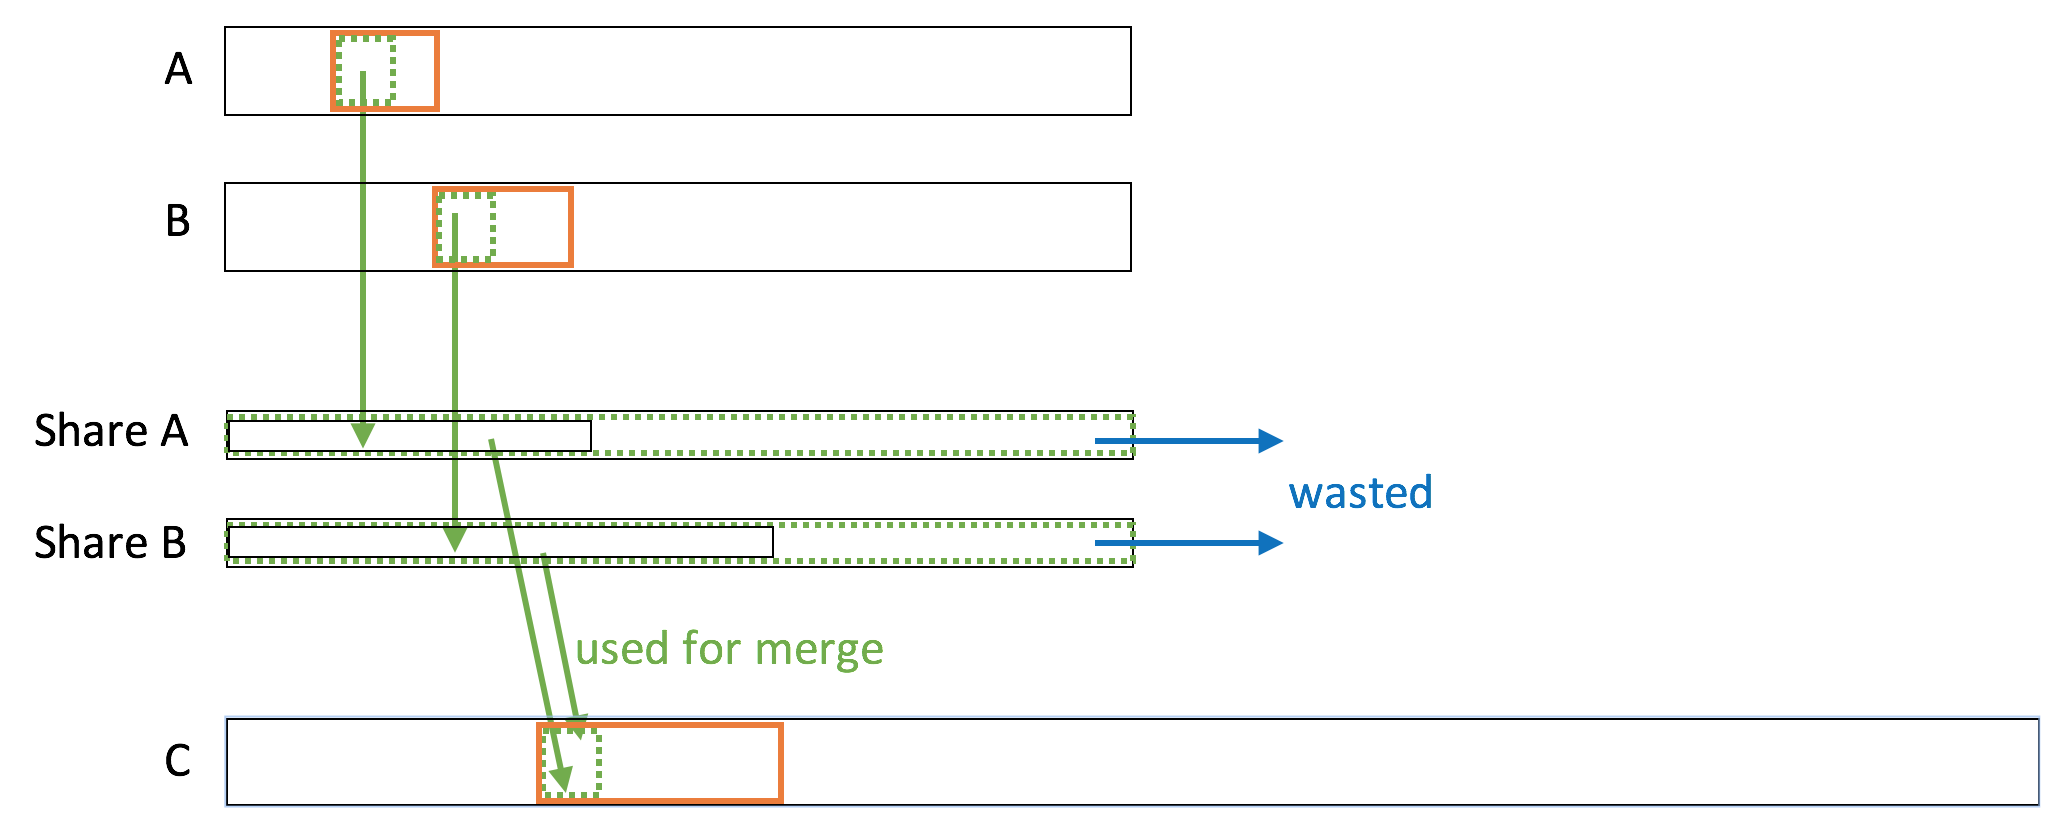
\includegraphics[width=\textwidth]{single1.png}
    \end{center}
    \caption{{\label{fig:single1}} First Iteration of Single Buffer Parallel Merge}
    \end{figure}

    In the next iteration, we will load the data we have not merged  
    into the shared memory, and do the same merge. 
    Figure \ref{fig:single2} shows the second iteration of single buffer
    parallel merge. The dashed red box is the second iteration of the thread level 
    run of co-rank function. 

    \begin{figure}[!h]
    \begin{center}
    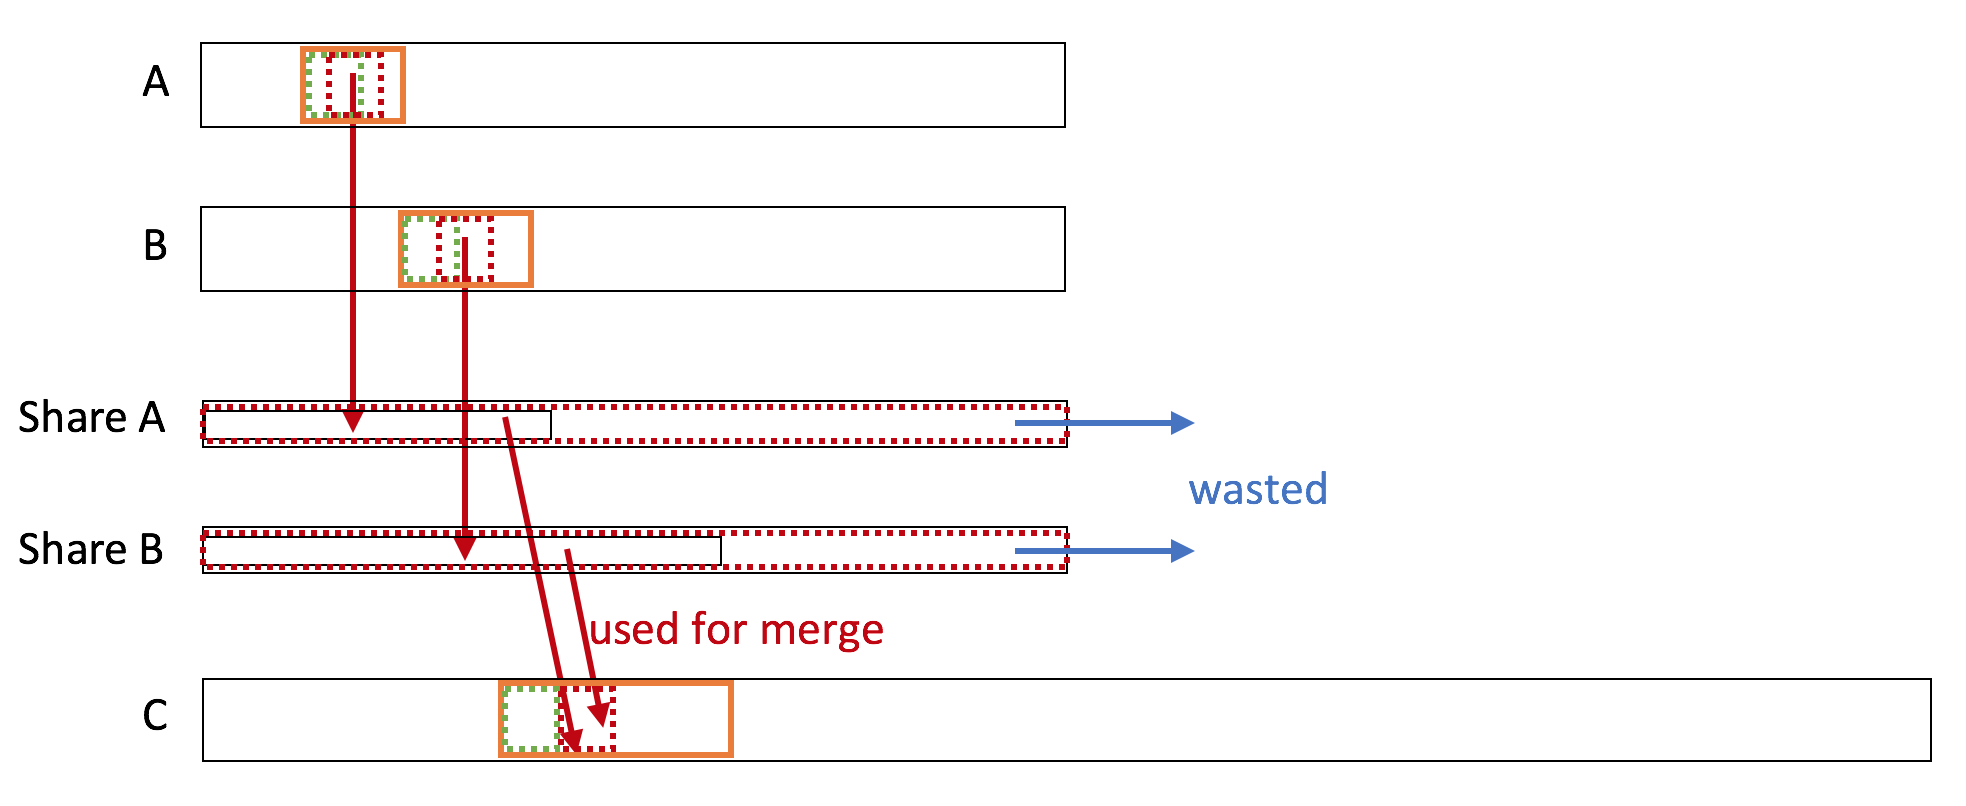
\includegraphics[width=\textwidth]{single2.png}
    \end{center}
    \caption{{\label{fig:single2}} Second Iteration of Single Buffer Parallel Merge}
    \end{figure}

    The loop runs until we have merged all the data that block is going to produce (filling 
    the entire solid orange box).   

    In single buffer parallel merge, we fill the shared memory in a coalesced pattern so that
    there will be fewer global memory requests. The thread level co-rank function runs on
    shared memory. The merge function reads the input from shared 
    memory, and writes to global memory. Because we convert many expensive global memory 
    reads to cheap shared memory
    reads, the single buffer parallel merge could better utilize the memory bandwidth and hence 
    outperform the naive parallel merge by 5x. 

    The performance of single buffer parallel merge is evaluated in Figure \ref{fig:single_evaluation}.

    \begin{figure}[!h]
    \begin{center}
    \resizebox{\textwidth}{!}{
        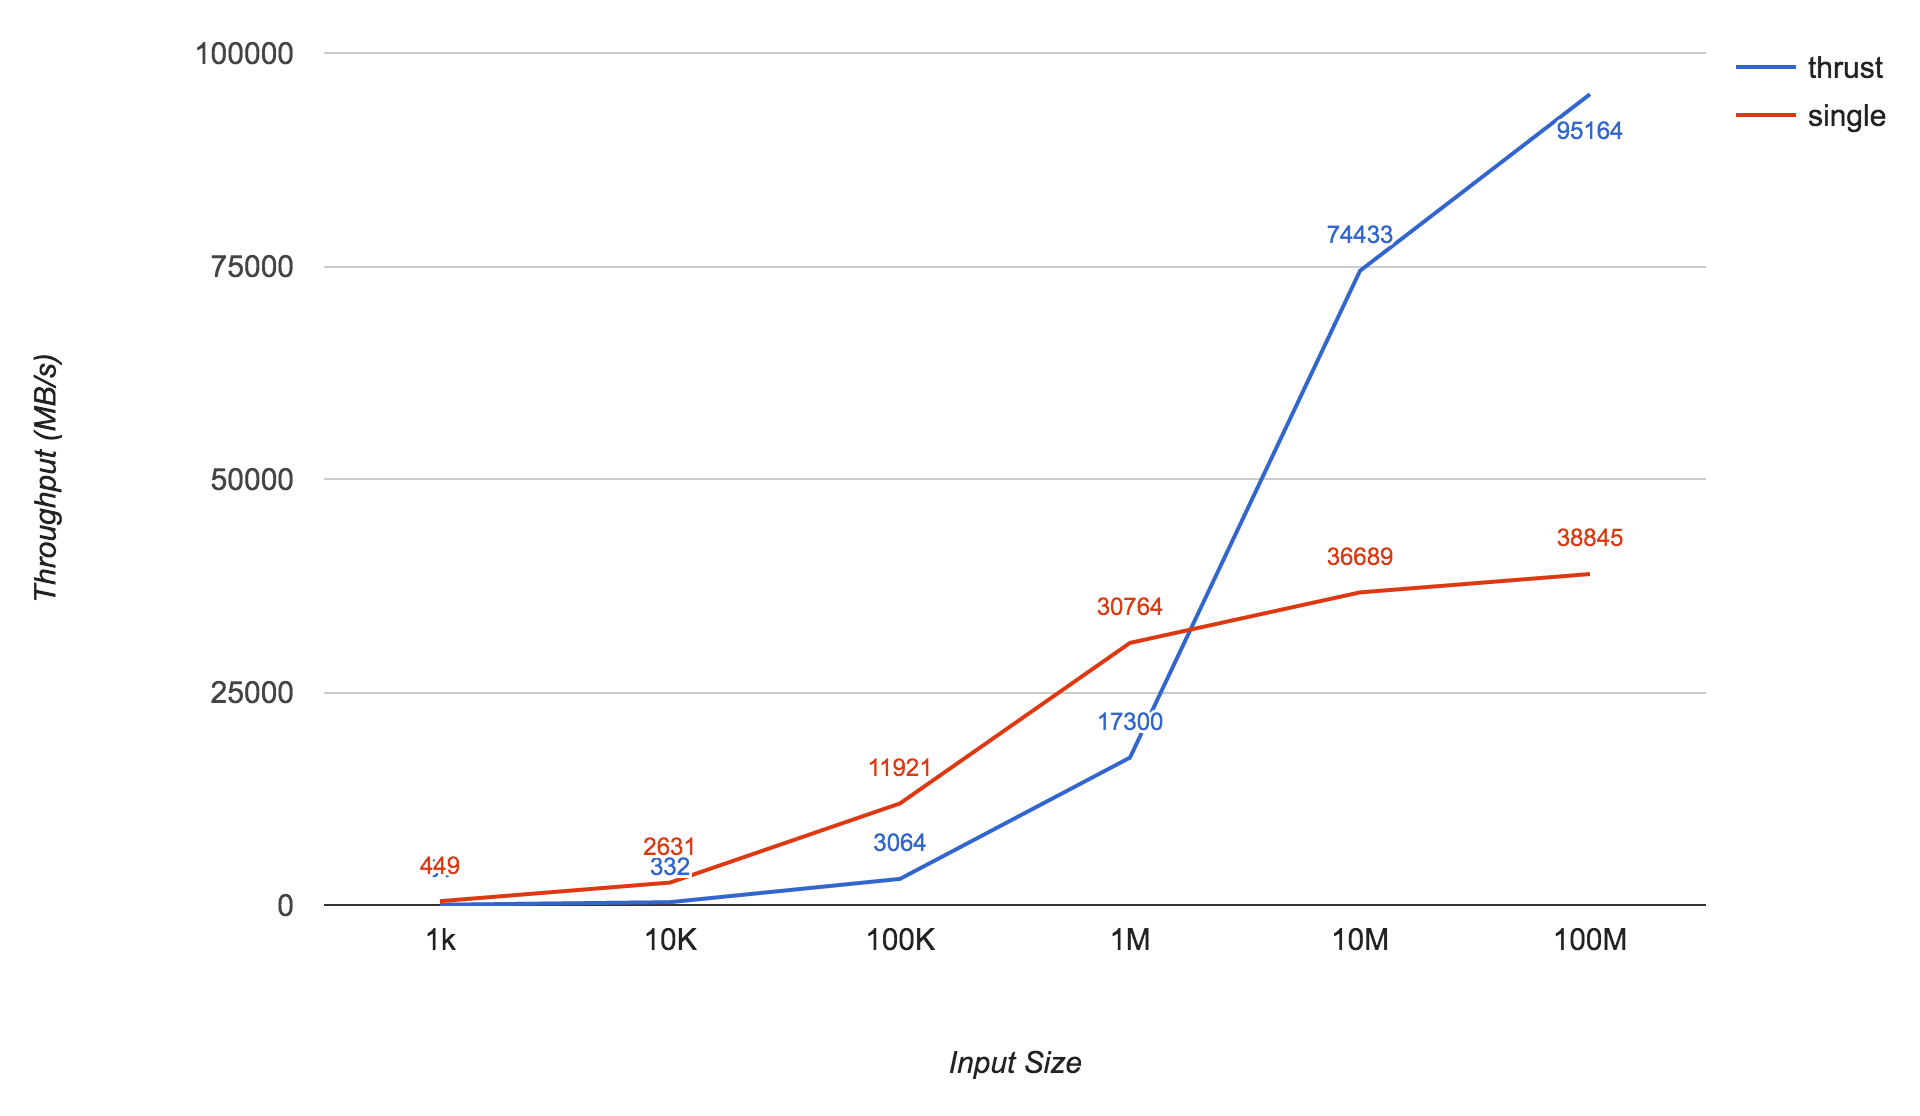
\includegraphics{single_evaluation.png}
    }
    \end{center}
    \caption{{\label{fig:single_evaluation}} Performance of Single Buffer Parallel Merge on Titan-Z}
    \end{figure}

%%%%%%%%%%%%%%%%%%%%%%%%%%%%%%%%%%%%%%%%%%%%%%%%%%%%%%%%%%%%%%%%
%   
%   Double Buffer Parallel Merge
%
    \section{Double Buffer Parallel Merge}\label{sect:double}
    In single buffer parallel merge, we only consume a half of the data we load into the shared 
    memory. The other half is wasted. To further 
    optimize the performance, we create the double buffer parallel merge, in which we 
    utilize all the data we load into the shared memory.

    The overall process is similar to single buffer parallel merge except for how we use
    shared memory. Co-rank function is
    run in two levels, block level and thread level. In the block level, all the threads in 
    the same block do the same searching. Each thread calculates the block index and total 
    number of blocks using $b\_id = blockIdx.x$ and $b\_num = gridDim.x$ respectively. 
    Based on $b\_id$ and $b\_num$, all threads within the same block calculate the output range 
    that block is going to produce, and use the output range as the input to the co-rank function 
    to identify the corresponding input ranges for that block. 
    After knowing the input ranges for the block, all threads in the block cooperatively load the 
    input to the shared memory.

    \begin{figure}[!h]
    \begin{center}
    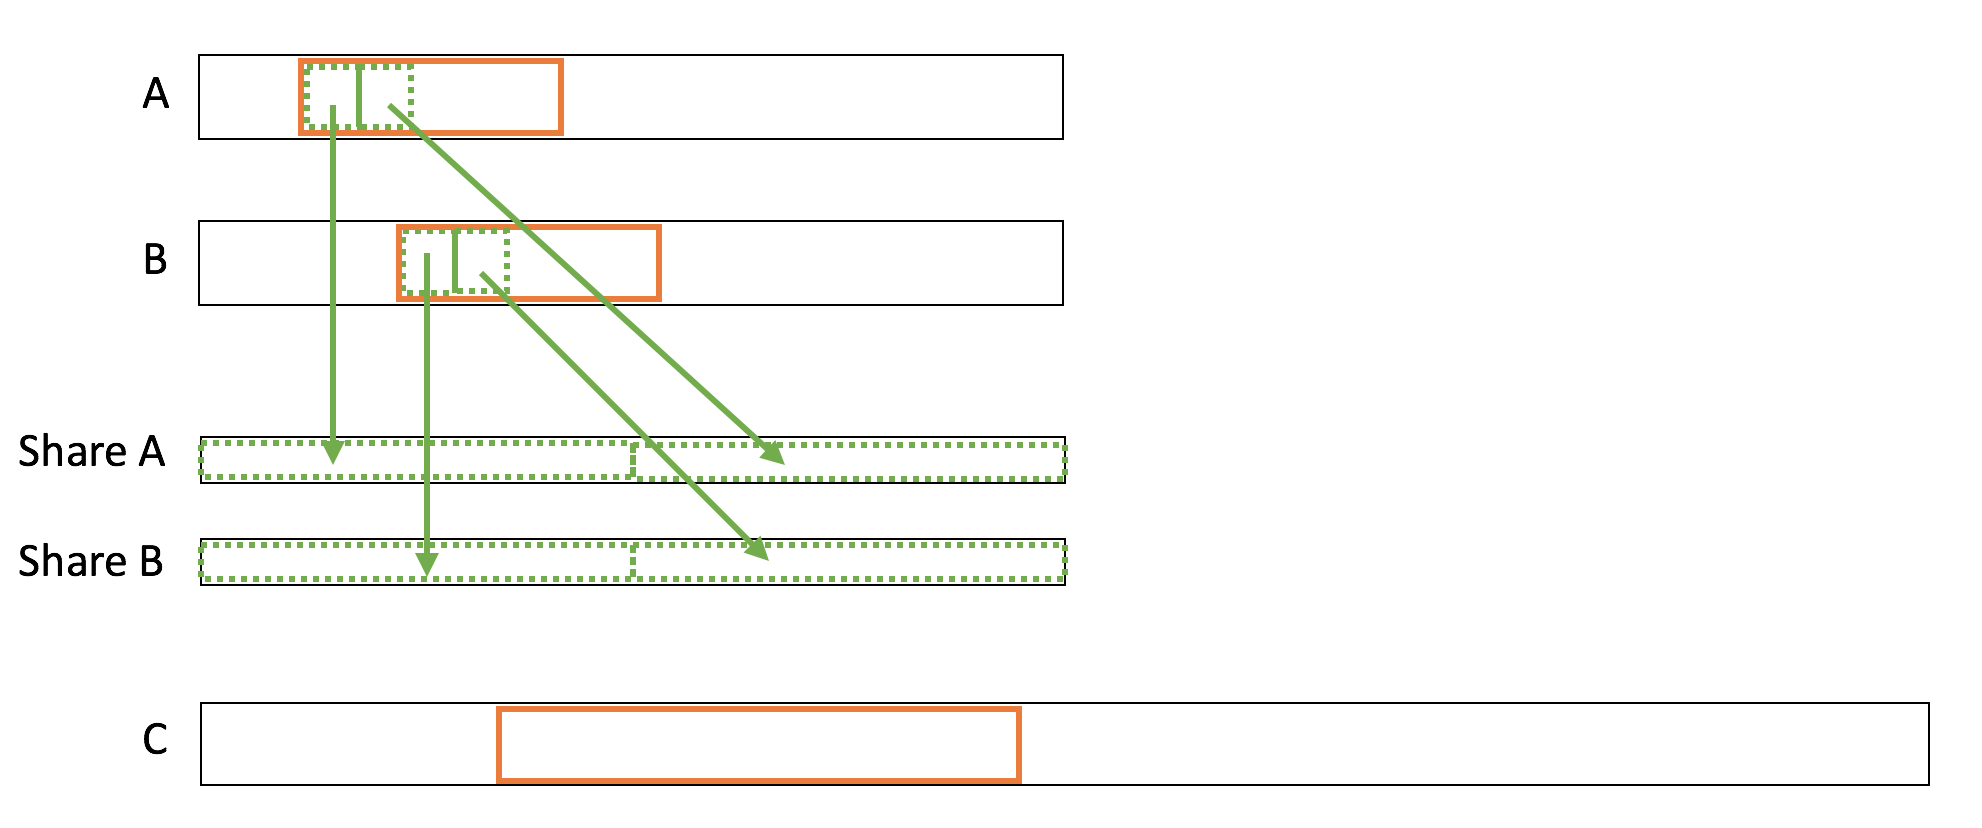
\includegraphics[width=\textwidth]{double0.png}
    \end{center}
    \caption{{\label{fig:double0}} Initialization of Double Buffer Parallel Merge}
    \end{figure}    

    We use a loop because shared memory may not be large enough to hold all the input data.
    When initializing, we load $2x$ elements from input array A and $2x$ elements from input 
    array B into the shared memory. Figure \ref{fig:double0} shows the initialization process.

    In each later iteration, all the threads in a block will produce $x$
    elements to the output array C. If there are more than $x$ elements in shared array A and 
    shared array B, we do not load from global memory. Figures \ref{fig:double1} and \ref{fig:double2} 
    show examples of the first iteration and second iteration of double buffer parallel 
    merge. In these two iterations, there are enough data remaining in the shared memory, 
    so we did not load from the global memory to shared memory.

    \begin{figure}[!h]
    \begin{center}
    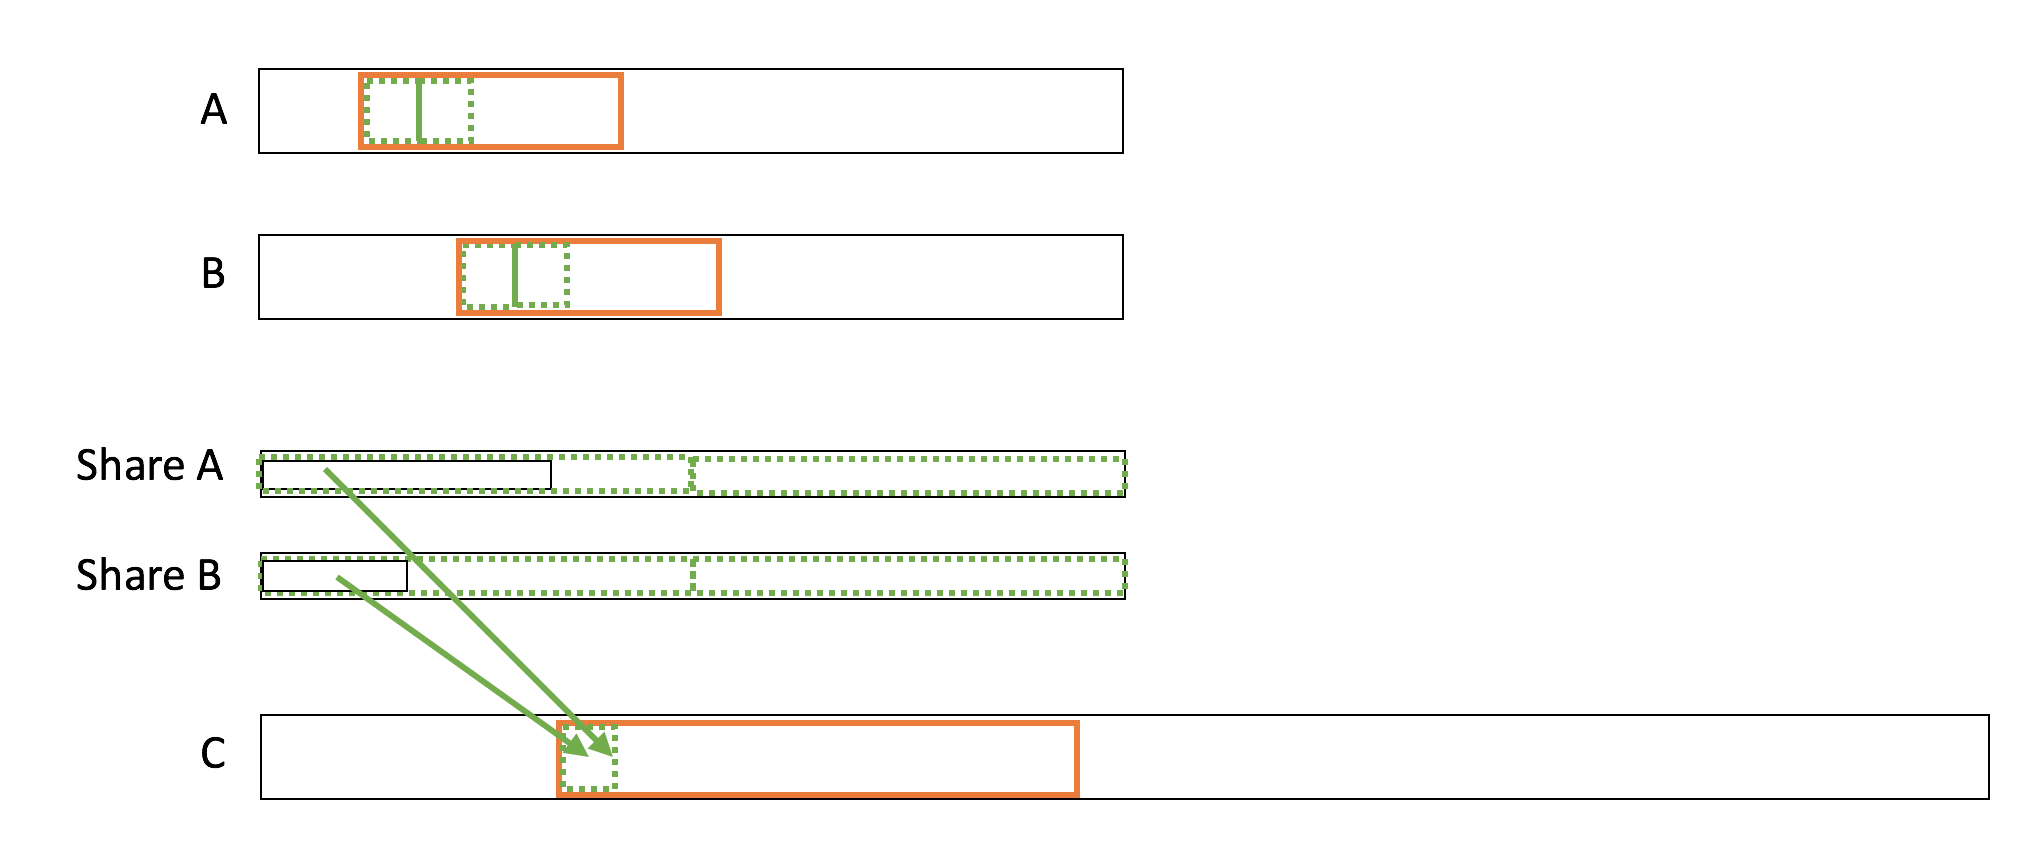
\includegraphics[width=\textwidth]{double1.png}
    \end{center}
    \caption{{\label{fig:double1}} First Iteration of Double Buffer Parallel Merge}
    \end{figure}

    \begin{figure}[!h]
    \begin{center}
    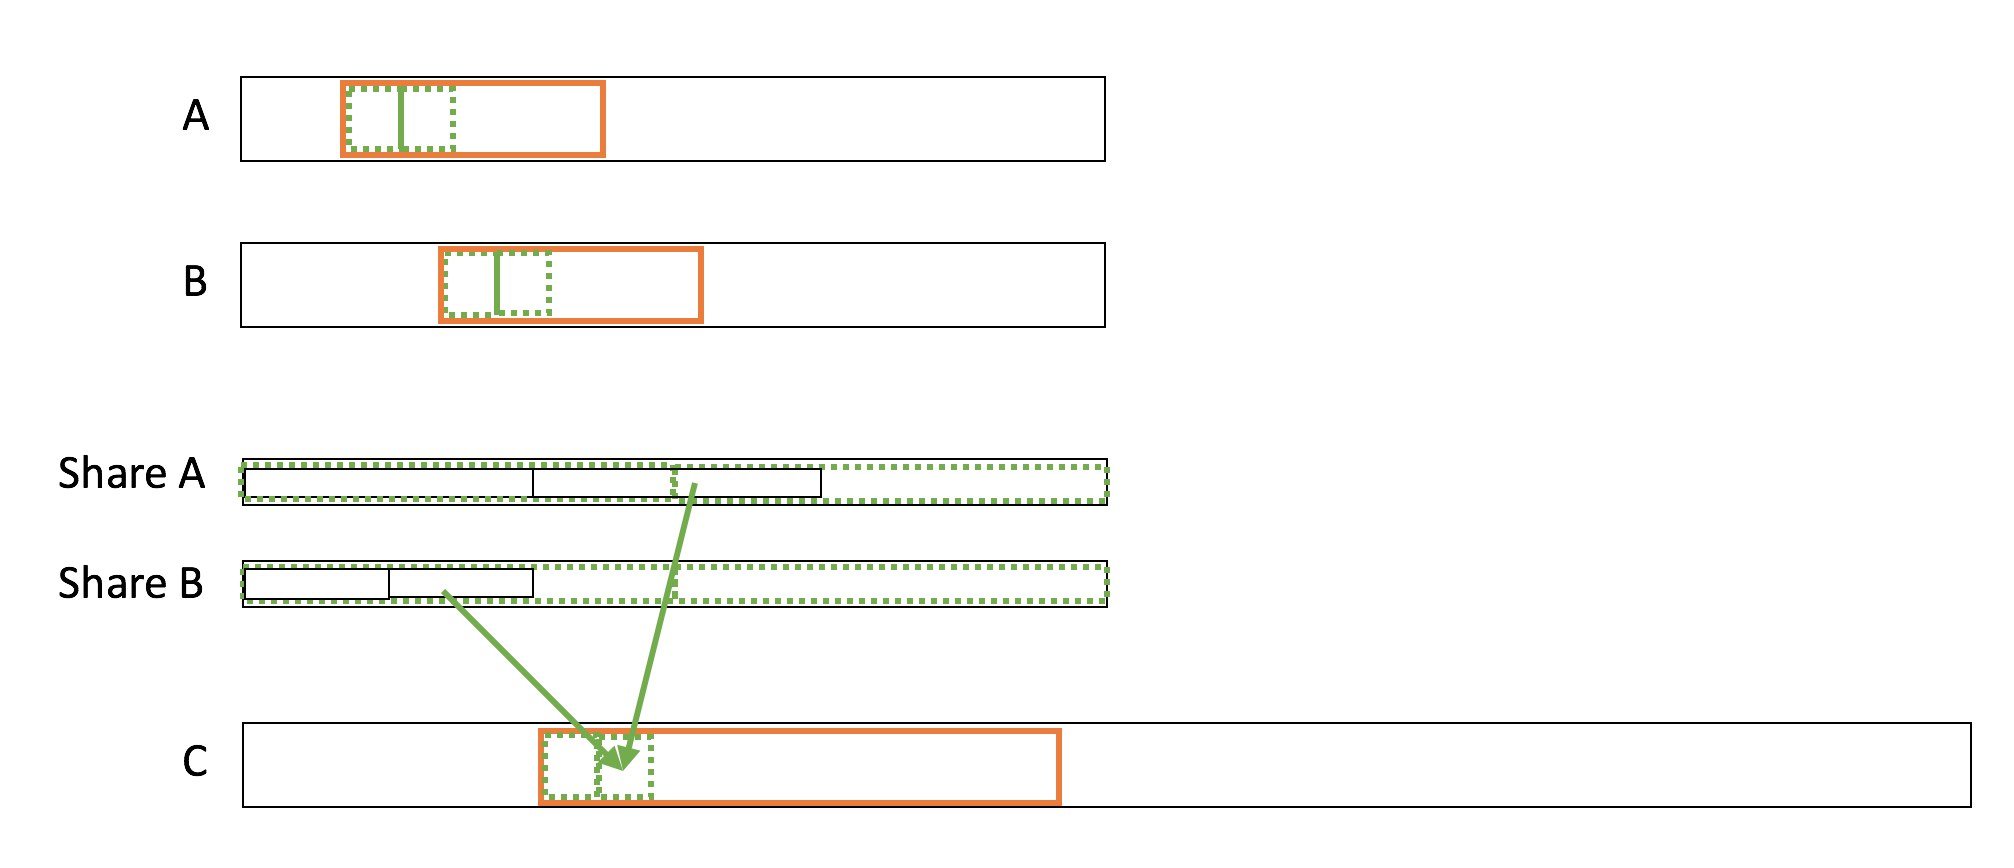
\includegraphics[width=\textwidth]{double2.png}
    \end{center}
    \caption{{\label{fig:double2}} Second Iteration of Double Buffer Parallel Merge}
    \end{figure}

    If there are less than $x$ elements in either shared array A or shared array B, 
    we will load another $x$ elements the into shared memory. Figure \ref{fig:double3} 
    shows an example of the third iteration of double buffer parallel 
    merge. In the third iteration, there are enough data in the shared array B. However,
    there are not enough (less than $x$) data in shared array A. So we load $x$ elements 
    from the global memory to shared memory (marked by the red box). Data in shared memory 
    will wrap around.  

    \begin{figure}[!h]
    \begin{center}
    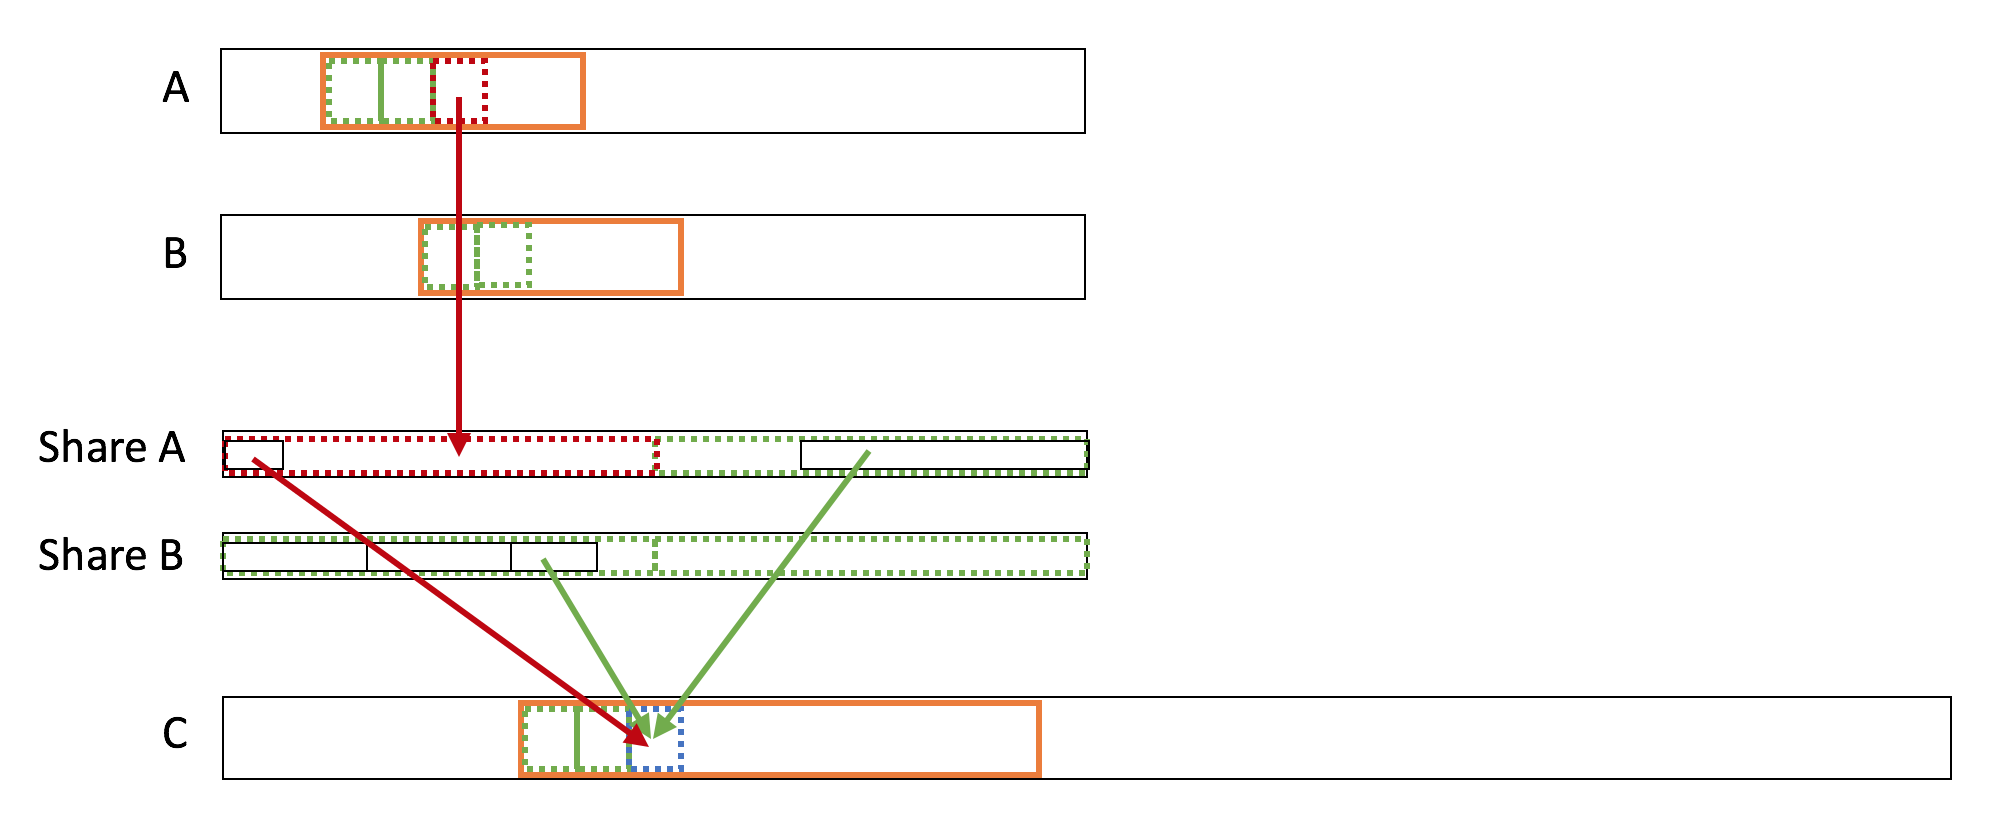
\includegraphics[width=\textwidth]{double3.png}
    \end{center}
    \caption{{\label{fig:double3}} Third Iteration of Double Buffer Parallel Merge}
    \end{figure}
 
    Then we run the co-rank function in thread level. The co-rank function is run on 
    shared memory. Each thread calculates the thread index and total number of threads 
    in the block using $t\_id = threadIdx.x$ and $r\_num = blockDim.x$ respectively. 
    Based on $t\_id$ and $t\_num$, each thread calculates the output range 
    that thread is going to produce, and uses the output range as the input to the co-rank function 
    to identify the corresponding input ranges.  
    Then each thread can start its work independently and call the sequential merge function to do 
    the merge in parallel on the input we load to shared memory and write the output to device 
    global memory.

    The loop runs until we have merged all the data that block is going to produce (filling 
    the entire solid orange box).   

    Notice that the memory access pattern of double buffer parallel merge is coalesced. 
    In double buffer parallel merge, we utilize all the 
    data we load into shared memory, while in single buffer parallel merge, we waste half of 
    the data we load into shared memory. We expect that double buffer parallel merge will 
    outperform single buffer parallel merge. However, in experiments, we observed that double 
    buffer used more registers (39) than single buffer parallel merge (31), and caused the occupancy 
    to drop. As a result, the double buffer parallel merge is not as fast as single buffer parallel
    merge. 

    The performance of double buffer parallel merge is evaluated in Figure \ref{fig:double_evaluation}.

    \begin{figure}[!h]
    \begin{center}
    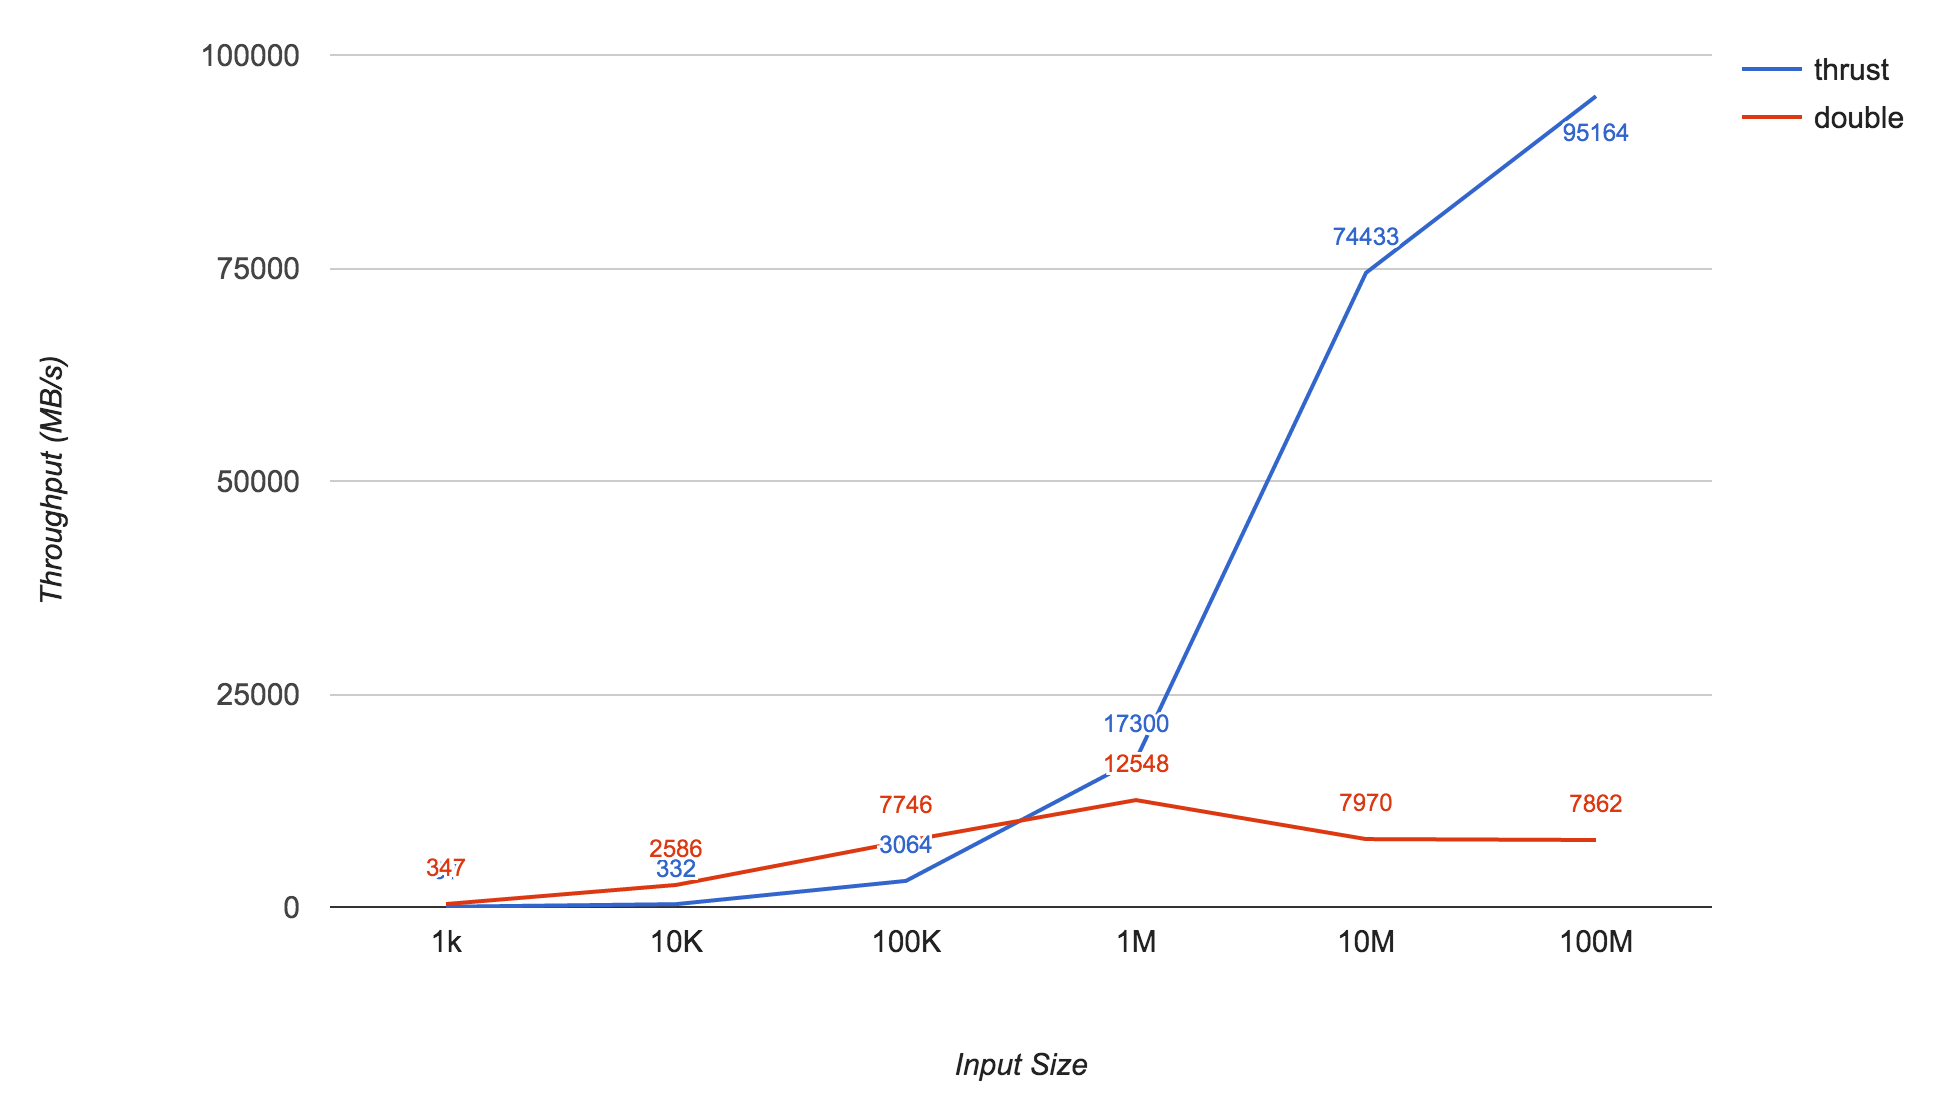
\includegraphics[width=\textwidth]{double_evaluation.png}
    \end{center}
    \caption{{\label{fig:double_evaluation}} Performance of Double Buffer Parallel Merge on Titan-Z}
    \end{figure}

%%%%%%%%%%%%%%%%%%%%%%%%%%%%%%%%%%%%%%%%%%%%%%%%%%%%%%%%%%%%%%%%
%   
%   Further Optimizations
%

    \section{Further Optimizations}\label{sect:opt}
        \subsection{Reduce Number of Calls to Co-rank Function}\label{sect:opt:co-rank}
        In all the GPU parallel merge implementations above, each thread needs to call the co-rank 
        function twice: once for the start point of the output range, and once for the end point 
        of the output range. Figure \ref{fig:reduce-0} gives an example. In this example, there 
        are $8$ threads. We mark the call to co-rank function using ``$*$". 
        Each thread will call co-rank twice to calculate $j\_start$ and $j\_end$.
        Therefore, the total number of calls to co-rank function is $16$.  

        \begin{figure}[!h]
        \begin{center}
        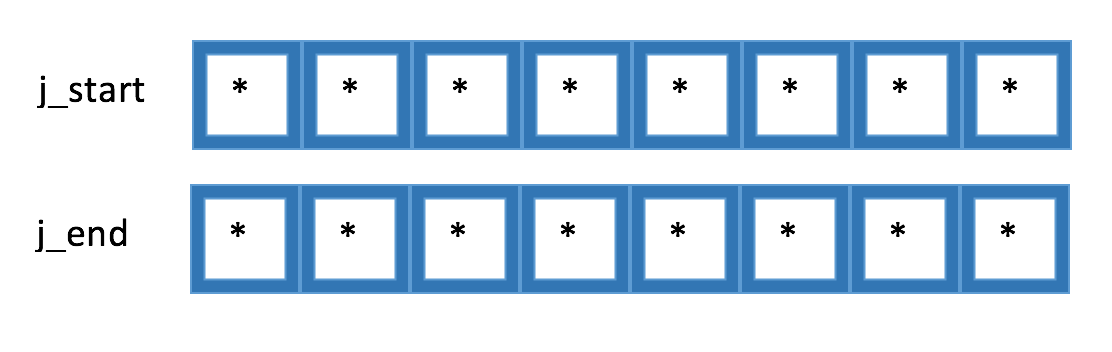
\includegraphics[width=\textwidth]{reduce-0.png}
        \end{center}
        \caption{{\label{fig:reduce-0}} Number of Calls to Co-rank Function}
        \end{figure}

        One observation we have is that the start point of thread $r$ is the same as 
        the end point of thread $r-1$. In the example we provide in figure \ref{fig:overall}, 
        the start point of $p1$ is $8$ and the end point of $p0$ is also $8$. 
        For this reason, we could reduce the number of calls to co-rank function. 
        We first let all the threads calculate the co-rank for the end point, 
        as shown in figure \ref{fig:reduce-1}.
        Instead of using co-rank function again to calculate the co-rank for starting point,
        we store the result($j\_end$) in an array in shared memory.  
        Then after a synchronization, we read the co-rank of start point of thread $r$
        from the result of thread $r-1$. If thread index is $0$, we will set the co-rank to $0$ 
        instead of reading from thread $-1$. Now we only need to call co-rank function for
        $8$ times (as marked by ``$*$" in figure \ref{fig:reduce-1}) and reduce the number of calls by half.     

        \begin{figure}[!h]
        \begin{center}
        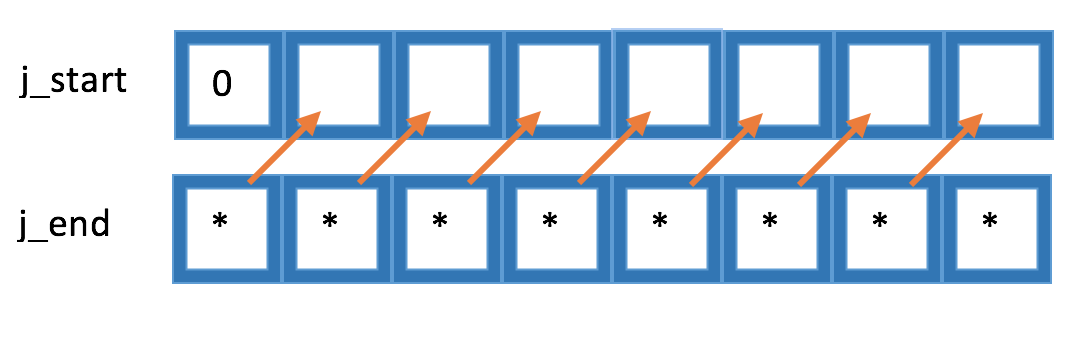
\includegraphics[width=\textwidth]{reduce-1.png}
        \end{center}
        \caption{{\label{fig:reduce-1}} Number of Calls to Co-rank Function after Optimization}
        \end{figure}


        \subsection{Change Code Divergence to Memory Divergence}\label{set:opt:div}
        Code divergence also hurts the performance of GPU application. When the threads in the 
        same warp take different branches for an $if-else$ statement, code divergence will occur.
        The hardware needs to execute the $if$ part and $else$ part sequentially. This will 
        hurt the overall performance. As a result, it is desirable 
        to write code with a minimum amount of code divergence to achieve high performance.
        In parallel merge, we are concerned about two functions: merge and co-rank.   
        \begin{itemize}
            \item Merge\\ 
                  Listing \ref{list:merge_origin} shows the original sequential merge code. 
                  It uses a while
                  loop to do the merge. It first merges A and B to C, and then copies the 
                  remaining A 
                  or B to C. We can see that the original merge has code divergence due to 
                  \textbf{if} and \textbf{else} statements inside the while loop. 
                  To remove the code divergence, we use \textbf{selection} to replace the 
                  \textbf{if} and \textbf{else} statements.
                  Listing  \ref{list:merge_nodiv} shows the sequential merge code after removing 
                  code divergence. After this optimization, we effectively replace all the code
                  divergence with memory divergence. 
            \item Co-rank\\
                  Listing \ref{list:corank_origin} shows the original code for co-rank function. 
                  The code divergence also comes from the \textbf{if} and \textbf{else} statements. We replace
                  the \textbf{if} and \textbf{else} statements by \textbf{selection}. The resulting code is 
                  shown in Listing \ref{list:corank_nodiv}.
        \end{itemize}

        \begin{minipage}{\linewidth}
        \begin{singlespace}
        \begin{lstlisting} [caption = {Merge Remove Code Divergence}, captionpos=b, label = {list:merge_nodiv}]
void merge(int *A, int m, int*B, int n, int*C) 
{
  int count = m+n;
  int ai = 0, bi=0;
  for(int i=0; i< count; ++i)
  {
    bool p;
    bool c1 = (bi >= n);
    bool c2 = (ai >= m);
    p = c1 ? true : c2 ? false : A[ai]>B[bi] ? false : true; 
    C[i] = p ? A[ai++] : B[bi++];
  }
}
        \end{lstlisting}
        \end{singlespace}
        \end{minipage}

        \begin{minipage}{\linewidth}
        \begin{singlespace}
        \begin{lstlisting} [caption = {Co-rank Remove Code Divergence}, captionpos=b, label = {list:corank_nodiv}]
int co_rank_j(int i, int* A, int m, int* B, int n)
{
    int j = i<m ? i : m;                //j = min(i,m)
    int k = i - j;
    int j_low = 0>(i-n) ? 0 : i-n;      //j_low = max(0, i-n) 
    int k_low;
    int delta;

    while(1)
    {
        bool cond_1 = j > 0 && k <n && A[j-1] > B[k];
        bool cond_2 = k > 0 && j <m && B[k-1] >= A[j];
        
        delta = cond_1 ? ((j-j_low-1)>>1) + 1 : 
                cond_2 ? ((k-k_low-1)>>1) + 1 : delta;
        k_low = cond_1 ? k : k_low;
        j_low = cond_2 ? j : j_low;
        j     = cond_1 ? j - delta : cond_2 ? j+delta : j;
        k     = cond_1 ? k + delta : cond_2 ? k-delta : k;
        if(!cond_1 && !cond_2)
            break;
    }
    return j;
}
        \end{lstlisting}
        \end{singlespace}
        \end{minipage}

        After removing code divergence, we see some speedup.

        Here is a figure.

    \section{Tuning Parameters}\label{sect:tuning}
    We set the number of blocks, the block dimension, and shared memory size as our tuning
    parameters.
    \begin{itemize}
    \item \textbf{number of blocks:} When we change the number of blocks, we are also changing
           the amount of work for each block. When we increase the number of blocks, we create 
           more parallelism that could be scheduled on different SM. Meanwhile, the amount of 
           work for each block is decreasing. We want the amount of work for each block to be
           large enough to amortize the block launch overhead. We choose the number of blocks 
           from 1, 4, 16, 64, 256, and 512.
    \item \textbf{block dimension:} Block dimension determines the number of threads in the 
           thread block. We choose the block dimension from 128, 256, and 512.
    \item \textbf{shared memory size:} Shared memory size can affect the number of blocks that
          can run simultaneously on the SM. We choose from 1024B, 2048B and 2560B. 
    \end{itemize}

    We enumerate all the combinations of tuning parameters, record their running time, and 
    choose the one that has the best performance.


